\subsection{Problem definition}

This work aims to study recurrent neural networks. However, it does not only focus on the theoretical section but also on the practical one. Therefore, a problem has been sought to be solved as an example. The problem which has been attempted to solve is the prediction of the demand of shared bicycles (bikesharing) in the city of Chicago. As a solution is to be carried out using supervised learning, a huge amount of data is needed beforehand. Chicago has been chosen for just that reason, because of the ease of access to public data needed to be able to train on the network without any restrictions or licences. In particular, the dataset offered by the company \textit{Divvy} has been downloaded \cite{divvy}.
\newline
 
In addition, the Chicago City Council offers interactive maps \cite{chicagomap} which have been of great help in studying the different properties of the stations, as well as a multitude of data providers, both meteorological \cite{chicagoweather} and of other types, which can also be added to the dataset and thus improve the precision of the model, but which, due to lack of time and the results obtained, could not be carried out as explained in section \ref{future_work}.
 

\begin{figure}[H]
    \centering
    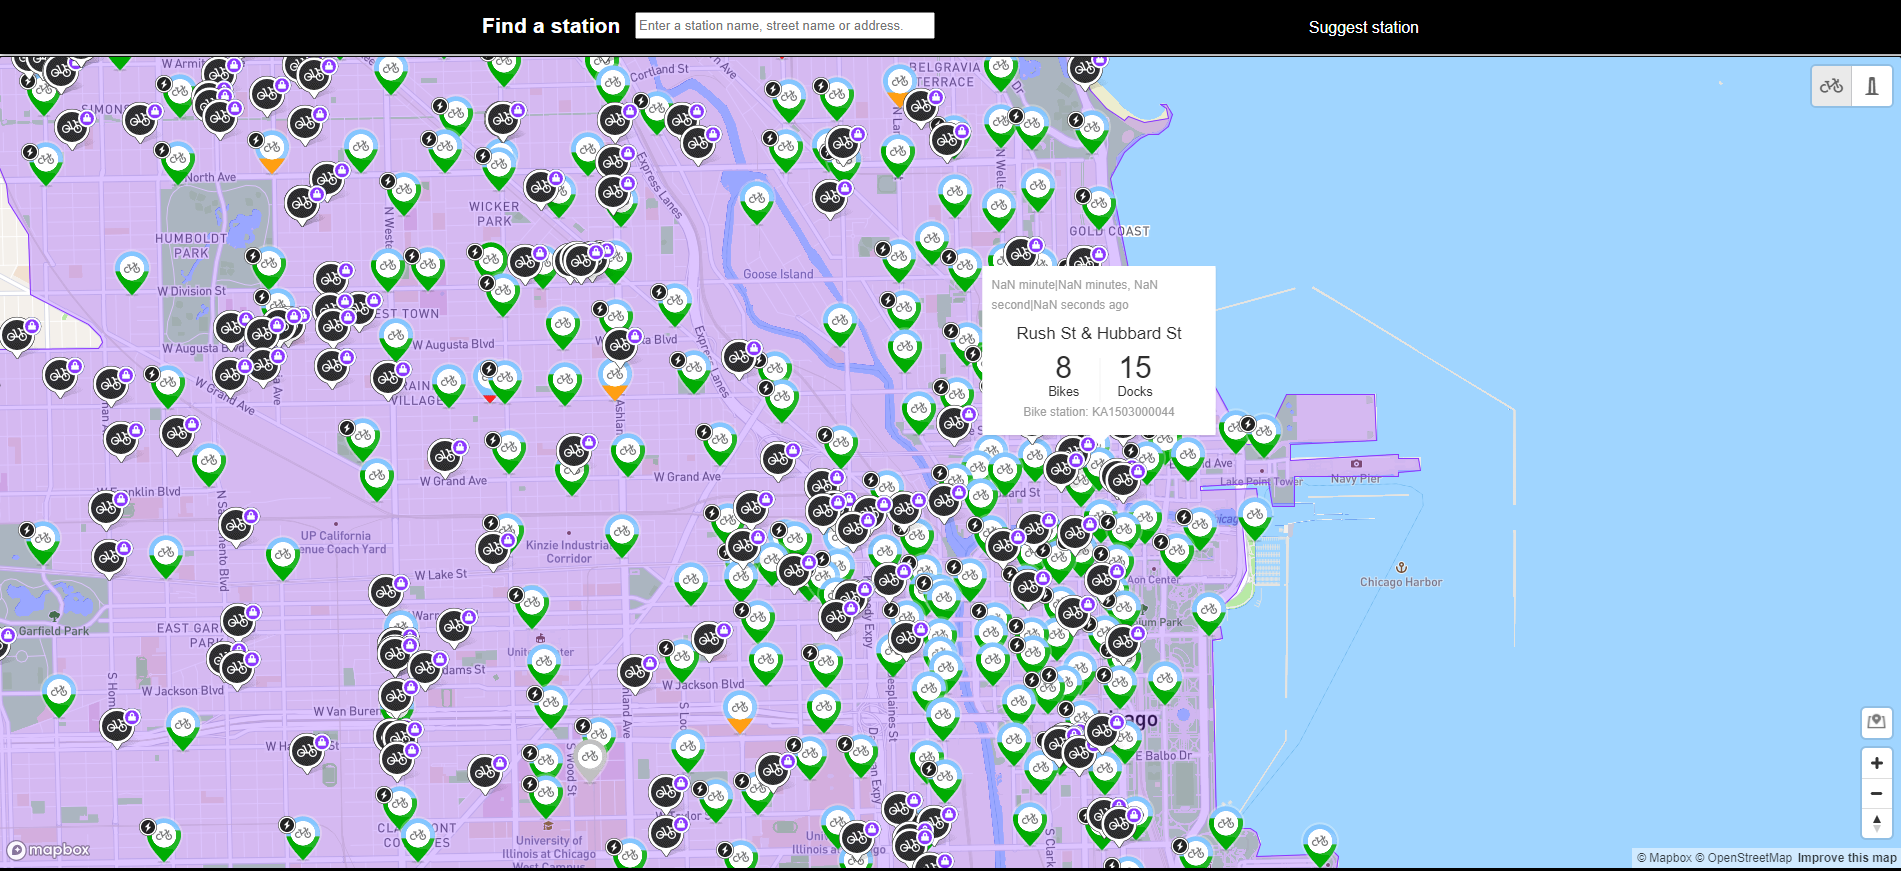
\includegraphics[width=14cm]{images/solution/preprocessing/divvy-map.png}
    \caption{Interactive map of the bike rental station network in Chicago \cite{chicagomap}}
\end{figure}
